\section{Baseline Forecasts}
In this section we present baseline forecasts of the Future Americans Model.  The figures show data from the PSID for the 25+ population from 1999 through 2009 and 
forecasts from the FAM for the 25+ population beginning in 2009.

\subsection{Disease Prevalence}
Figure \ref{fig:chronic_diseases_male} depicts the six chronic conditions we project for men.  And Figure \ref{fig:chronic_diseases_female} depicts the historic 
and forecasted values for women.

\begin{figure}[ht!]
\centering

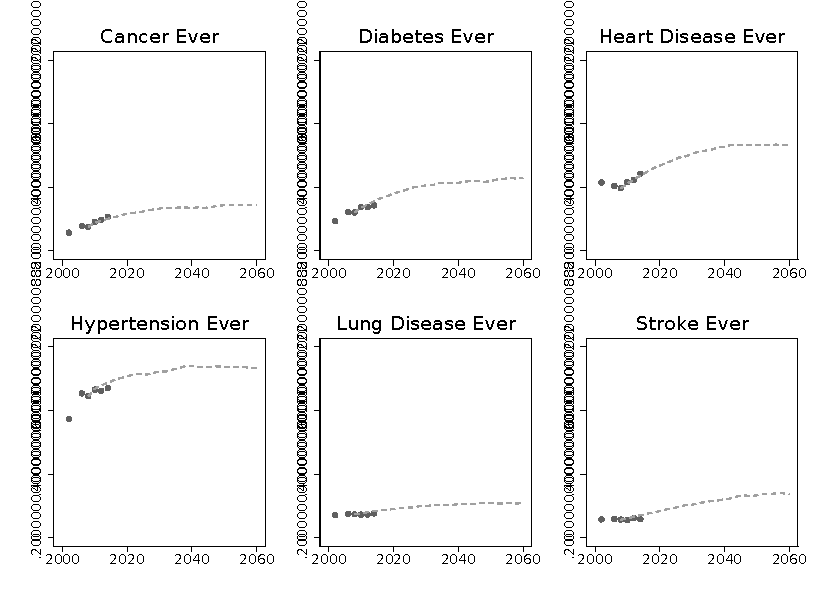
\includegraphics[scale=1.0]{./img/chronic_diseases_male}
\caption{Historic and Forecasted Chronic Disease Prevalence for Men 25+}
\label{fig:chronic_diseases_male} 

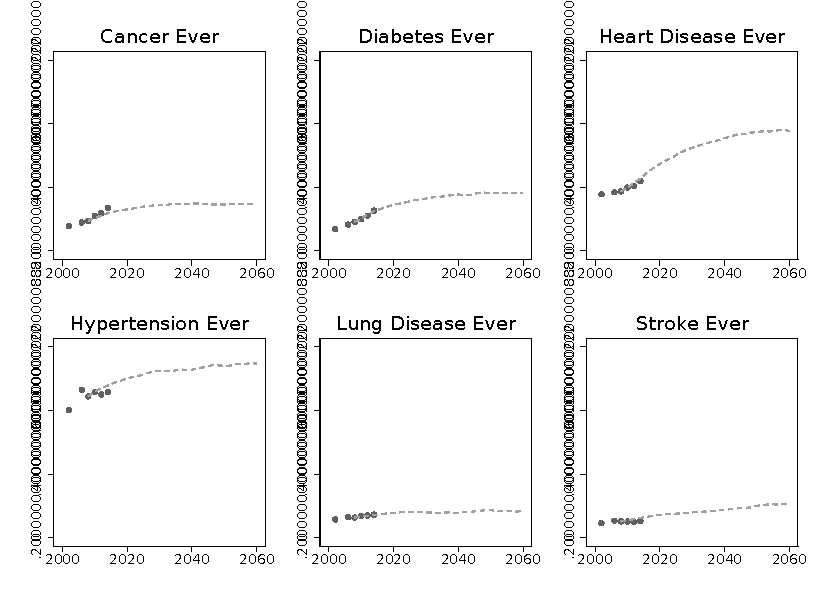
\includegraphics[scale=1.0]{./img/chronic_diseases_female}
\caption{Historic and Forecasted Chronic Disease Prevalence for Women 25+}
\label{fig:chronic_diseases_female} 
\end{figure}

Figure \ref{fig:adl_iadl_male} shows historic and forecasted levels for any ADL difficulties, three or more ADL difficulties, any IADL difficulties, and
two or more IADL difficulties for men 25 and older. Figure \ref{fig:adl_iadl_female} shows historic and forecasted levels for any ADL difficulties, three or 
more ADL difficulties, any IADL difficulties, and two or more IADL difficulties for women 25 and older.

\begin{figure}[ht!]
\centering

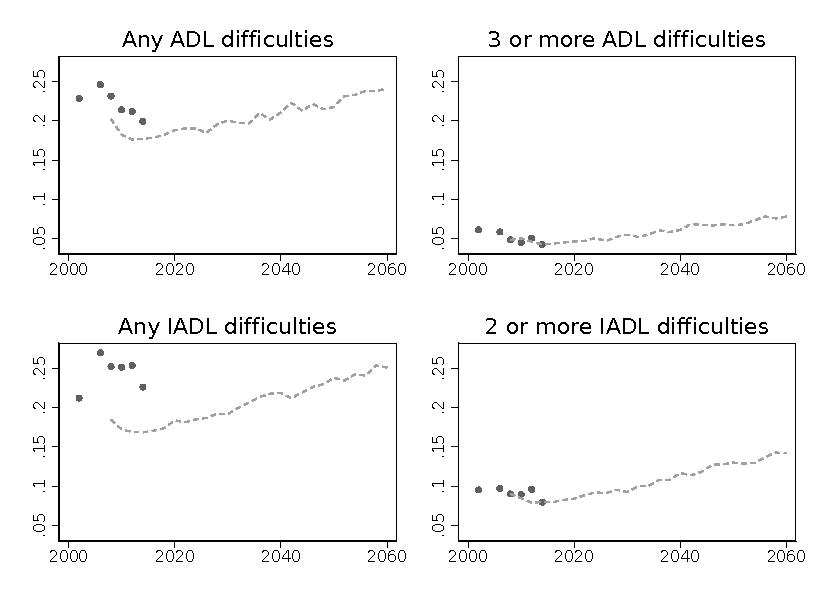
\includegraphics[scale=1.0]{./img/adl_iadl_male}
\caption{Historic and Forecasted ADL and IADL Prevalence for Men 25+}
\label{fig:adl_iadl_male} 

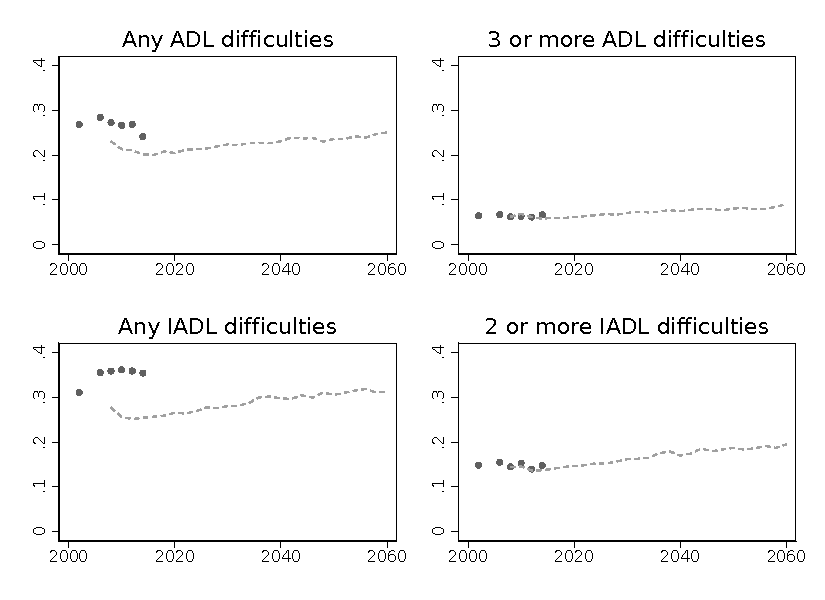
\includegraphics[scale=1.0]{./img/adl_iadl_female}
\caption{Historic and Forecasted ADL and IADL Prevalence for Women 25+}
\label{fig:adl_iadl_female} 
\end{figure}
